\documentclass[11pt]{beamer}
\usetheme{Copenhagen}
\usepackage{tikz}
\usetikzlibrary{calc}

% set captions with numbers
\setbeamertemplate{caption}[numbered]

\usepackage{tikz-3dplot}

\usepackage{amssymb}

\usepackage{xcolor}

%--------------------------------------------------------------------
% To get rid of the bottom navigation bars:
\setbeamertemplate{footline}[frame number]{}

% To get rid of the bottom navigation symbols:
\setbeamertemplate{navigation symbols}{}

% To get rid of the footer:
\setbeamertemplate{footline}{}

%--------------------------------------------------------------------
\title{Kochen-Specker Uncolorable Sets:}
\subtitle{An Algorithmic Approach to Proving Contradictions}
\author{Camilo Morales}
\institute{Department of Mathematics \\ University of California, Irvine}
\date{}

\begin{document}
         
\frame{\titlepage}

%--------------------------------------------------------------------
\begin{frame}{Vector Spaces}

\pause

\begin{columns}
	
	\begin{column}{0.45\textwidth}
	
		\begin{figure}[htp]
			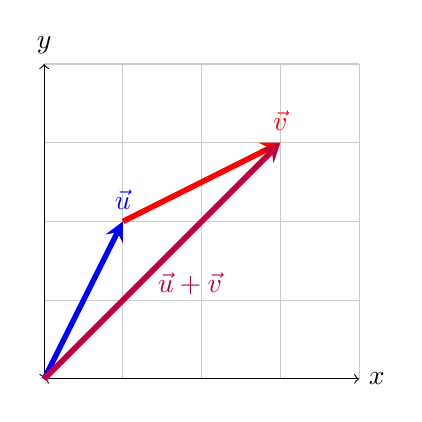
\begin{tikzpicture}
  				\draw[thin, gray!40] (0, 0) grid (4, 4);
  				\draw[<->] (0, 0)--(4, 0) node[right]{$x$};
  				\draw[<->] (0, 0)--(0, 4) node[above]{$y$};
  				\draw[line width = 2pt, blue, -stealth] (0, 0) -- (1, 2) node[anchor = south]{$\vec{u}$};
  				\draw[line width = 2pt, red, -stealth] (1, 2) -- (3, 3) node[anchor = south]{$\vec{v}$};
  				\draw[line width = 2pt, purple, -stealth] let \p1 = (0, 0),
  											 \p2 = (3, 3) in
											 (\p1) -- (\p2) node at ({(\x2 / 2) + 10}, \y2 / 2) [anchor = north]{$\vec{u} + \vec{v}$};
			\end{tikzpicture}

			\caption{Vector addition}

		\end{figure}
		
	\end{column}
	
	\begin{column}{0.45\textwidth}
	
		\begin{figure}[htp]
			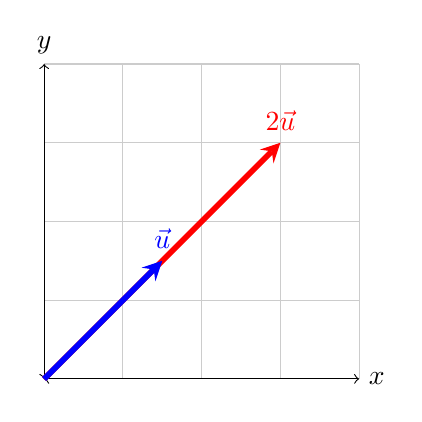
\begin{tikzpicture}
  				\draw[thin, gray!40] (0, 0) grid (4, 4);
  				\draw[<->] (0, 0)--(4, 0) node[right]{$x$};
  				\draw[<->] (0, 0)--(0, 4) node[above]{$y$};
  				\draw[line width = 2pt, red, -stealth] (0, 0) -- (3, 3) node[anchor = south]{$2 \vec{u}$};
  				\draw[line width = 2pt, blue, -stealth] (0, 0) -- (1.5, 1.5) node[anchor = south]{$\vec{u}$};
			\end{tikzpicture}
						
			\caption{Scalar multiplication}
				
		\end{figure}
		
	\end{column}
	
\end{columns}

\end{frame}

%--------------------------------------------------------------------
\begin{frame}{Orthogonality}

\centering

\begin{figure}[htp]
	\tdplotsetmaincoords{60}{110}
	\begin{tikzpicture}[scale = 2,tdplot_main_coords]

		\draw[thick,->] (0, 0, 0) -- (2, 0, 0) node[below left = -3]{$x$};
		\draw[thick,->] (0, 0, 0) -- (0, 2, 0) node[right = -1]{$y$};
		\draw[thick,->] (0, 0, 0) -- (0, 0, 2) node[above = -1]{$z$};
	
		\draw[line width = 2pt, blue, -stealth] (0, 0, 0) -- (1.5, 0, 0) node[anchor = south east]{$\vec{v_{1}}$};
		\draw[line width = 2pt, red, -stealth] (0, 0, 0) -- (0, 1.5, 0) node[anchor = south west]{$\vec{v_{2}}$};
		\draw[line width = 2pt, purple, -stealth] (0, 0, 0) -- (0, 0, 1.5) node[anchor = south east]{$\vec{v_{3}}$};

		\draw[thick, dashed, black] (0.5, 0, 0) -- (0.5, 0, 0.5);
		\draw[thick, dashed, black] (0.5, 0, 0.5) -- (0, 0, 0.5);
	
		\draw[thick, dashed, black] (0, 0, 0.5) -- (0, 0.5, 0.5);
		\draw[thick, dashed, black] (0, 0.5, 0.5) -- (0, 0.5, 0);

		\draw[thick, dashed, black] (0, 0.5, 0) -- (0.5, 0.5, 0);	
		\draw[thick, dashed, black] (0.5, 0.5, 0) -- (0.5, 0, 0);
	\end{tikzpicture}

	\caption{$\vec{v_{1}}$, $\vec{v_{2}}$, and $\vec{v_{3}}$ are pairwise orthogonal.}
				
\end{figure}

\end{frame}

%------------------------------------------------------------------
\begin{frame}{Orthogonality}

\begin{center}

	\tdplotsetmaincoords{60}{110}
	\begin{tikzpicture}[scale = 2,tdplot_main_coords]

		\draw[thick,->] (0, 0, 0) -- (1.5, 0, 0) node[below left = -3]{$x$};
		\draw[thick,->] (0, 0, 0) -- (0, 1.5, 0) node[right = -1]{$y$};
		\draw[thick,->] (0, 0, 0) -- (0, 0, 1.5) node[above = -1]{$z$};
	
		\draw[line width = 2pt, blue, -stealth] (0, 0, 0) -- (1, 0, 0) node[anchor = south east]{$(1, 0, 0)$};
		\draw[line width = 2pt, red, -stealth] (0, 0, 0) -- (0, 1, 0) node[anchor = south west]{$(0, 1, 0)$};
		\draw[line width = 2pt, purple, -stealth] (0, 0, 0) -- (0, 0, 1) node[anchor = south east]{$(0, 0, 1)$};

		\draw[thick, dashed, black] (0.25, 0, 0) -- (0.25, 0, 0.25);
		\draw[thick, dashed, black] (0.25, 0, 0.25) -- (0, 0, 0.25);
	
		\draw[thick, dashed, black] (0, 0, 0.25) -- (0, 0.25, 0.25);
		\draw[thick, dashed, black] (0, 0.25, 0.25) -- (0, 0.25, 0);

		\draw[thick, dashed, black] (0, 0.25, 0) -- (0.25, 0.25, 0);	
		\draw[thick, dashed, black] (0.25, 0.25, 0) -- (0.25, 0, 0);
	\end{tikzpicture}
	
\end{center}
	
\pause
	
Computing the dot product of each pair of vectors above will always yield 0:
\[\begingroup\color{blue}{(1, 0, 0)}\endgroup \cdot \begingroup\color{red}{(0, 1, 0)}\endgroup = (\begingroup\color{blue}{1}\endgroup \cdot \begingroup\color{red}{0}\endgroup) + (\begingroup\color{blue}{0}\endgroup \cdot \begingroup\color{red}{1}\endgroup) + (\begingroup\color{blue}{0}\endgroup \cdot \begingroup\color{red}{0}\endgroup) = 0 + 0 + 0 = 0.\]
		
\end{frame}

%------------------------------------------------------------------
\begin{frame}{Orthogonal Sets}

\begin{block}{Definition}
	A set of vectors $\{\vec{v_{1}}, \vec{v_{2}}, \dots, \vec{v_{k}}\}$ in a vector space $V$ is called an \textbf{orthogonal set} if all pairs of distinct vectors in the set are orthogonal -- that is, if
	\[\vec{v_{i}} \cdot \vec{v_{j}} = 0 \quad \text{whenever} \quad i \neq j \text{ for } i, j = 1, 2, \dots, k.\]
\end{block}
		
\end{frame}

%------------------------------------------------------------------
\begin{frame}{Coloring and Contextuality}

\centering

\tdplotsetmaincoords{60}{110}
\begin{tikzpicture}[scale = 2,tdplot_main_coords]

	\draw[thick,->] (0, 0, 0) -- (2, 0, 0) node[below left = -3]{$x$};
	\draw[thick,->] (0, 0, 0) -- (0, 2, 0) node[right = -1]{$y$};
	\draw[thick,->] (0, 0, 0) -- (0, 0, 2) node[above = -1]{$z$};
	
	\draw[line width = 2pt, gray, -stealth] (0, 0, 0) -- (1.5, 0, 0) node[anchor = south east]{$\vec{v_{1}}$};
	\draw[line width = 2pt, gray, -stealth] (0, 0, 0) -- (0, 1.5, 0) node[anchor = south west]{$\vec{v_{2}}$};
	\draw[line width = 2pt, gray, -stealth] (0, 0, 0) -- (0, 0, 1.5) node[anchor = south east]{$\vec{v_{3}}$};

	\draw[thick, dashed, black] (0.5, 0, 0) -- (0.5, 0, 0.5);
	\draw[thick, dashed, black] (0.5, 0, 0.5) -- (0, 0, 0.5);
	
	\draw[thick, dashed, black] (0, 0, 0.5) -- (0, 0.5, 0.5);
	\draw[thick, dashed, black] (0, 0.5, 0.5) -- (0, 0.5, 0);

	\draw[thick, dashed, black] (0, 0.5, 0) -- (0.5, 0.5, 0);	
	\draw[thick, dashed, black] (0.5, 0.5, 0) -- (0.5, 0, 0);
\end{tikzpicture}

\end{frame}

%------------------------------------------------------------------
\begin{frame}{Coloring and Contextuality}

\centering

\tdplotsetmaincoords{60}{110}
\begin{tikzpicture}[scale = 2,tdplot_main_coords]

	\draw[thick,->] (0, 0, 0) -- (2, 0, 0) node[below left = -3]{$x$};
	\draw[thick,->] (0, 0, 0) -- (0, 2, 0) node[right = -1]{$y$};
	\draw[thick,->] (0, 0, 0) -- (0, 0, 2) node[above = -1]{$z$};
	
	\draw[line width = 2pt, blue, -stealth] (0, 0, 0) -- (1.5, 0, 0) node[anchor = south east]{$\vec{v_{1}}$};
	\draw[line width = 2pt, blue, -stealth] (0, 0, 0) -- (0, 1.5, 0) node[anchor = south west]{$\vec{v_{2}}$};
	\draw[line width = 2pt, red, -stealth] (0, 0, 0) -- (0, 0, 1.5) node[anchor = south east]{$\vec{v_{3}}$};

	\draw[thick, dashed, black] (0.5, 0, 0) -- (0.5, 0, 0.5);
	\draw[thick, dashed, black] (0.5, 0, 0.5) -- (0, 0, 0.5);
	
	\draw[thick, dashed, black] (0, 0, 0.5) -- (0, 0.5, 0.5);
	\draw[thick, dashed, black] (0, 0.5, 0.5) -- (0, 0.5, 0);

	\draw[thick, dashed, black] (0, 0.5, 0) -- (0.5, 0.5, 0);	
	\draw[thick, dashed, black] (0.5, 0.5, 0) -- (0.5, 0, 0);
\end{tikzpicture}

\end{frame}

%----------------------------------------------------------------
\begin{frame}{The Kochen-Specker (KS) Theorem}

\begin{block}{Kochen-Specker, 1967}
	There is a finite set $\mathcal{S} \subset \mathbb{R}^{3}$ such that there is no function $f: \mathcal{S} \to \{\begingroup\color{blue}{0}\endgroup, \begingroup\color{red}{1}\endgroup\}$ satisfying
	\[f(\vec{u}) + f(\vec{v}) + f(\vec{w}) = \begingroup\color{red}{1}\endgroup\]
	for all triples $(\vec{u}, \vec{v}, \vec{w})$ of mutually orthogonal vectors in $\mathcal{S}$.
\end{block}

\vfill

$\mathbb{R}^{3} := \{(x, y, z) : x, y, z \in \mathbb{R}\}$

\end{frame}

%----------------------------------------------------------------
\begin{frame}{The Kochen-Specker (KS) Theorem}

Let $\mathcal{S}$ be a set of vectors and consider the value function $f: \mathcal{S} \to \{\begingroup\color{blue}{0}\endgroup, \begingroup\color{red}{1}\endgroup\}$.

\pause

\centering

\tdplotsetmaincoords{60}{110}
\begin{tikzpicture}[scale = 2,tdplot_main_coords]

	\draw[thick,->] (0, 0, 0) -- (2, 0, 0) node[below left = -3]{$x$};
	\draw[thick,->] (0, 0, 0) -- (0, 2, 0) node[right = -1]{$y$};
	\draw[thick,->] (0, 0, 0) -- (0, 0, 2) node[above = -1]{$z$};
	
	\draw[line width = 2pt, blue, -stealth] (0, 0, 0) -- (1.5, 0, 0) node[anchor = south east]{$\vec{v_{1}}$};
	\draw[line width = 2pt, blue, -stealth] (0, 0, 0) -- (0, 1.5, 0) node[anchor = south west]{$\vec{v_{2}}$};
	\draw[line width = 2pt, red, -stealth] (0, 0, 0) -- (0, 0, 1.5) node[anchor = south east]{$\vec{v_{3}}$};

	\draw[thick, dashed, black] (0.5, 0, 0) -- (0.5, 0, 0.5);
	\draw[thick, dashed, black] (0.5, 0, 0.5) -- (0, 0, 0.5);
	
	\draw[thick, dashed, black] (0, 0, 0.5) -- (0, 0.5, 0.5);
	\draw[thick, dashed, black] (0, 0.5, 0.5) -- (0, 0.5, 0);

	\draw[thick, dashed, black] (0, 0.5, 0) -- (0.5, 0.5, 0);	
	\draw[thick, dashed, black] (0.5, 0.5, 0) -- (0.5, 0, 0);
\end{tikzpicture}

\[f(\vec{v_{1}}) = \begingroup\color{blue}{0}\endgroup \quad f(\vec{v_{2}}) = \begingroup\color{blue}{0}\endgroup \quad f(\vec{v_{3}}) = \begingroup\color{red}{1}\endgroup\]
\end{frame}

%-------------------------------------------------------------------
\begin{frame}{The Kochen-Specker (KS) Theorem}

\centering

\begin{figure}
	\includegraphics[width=0.65 \textwidth]{Kochen-Specker sets}
	
	\caption{A graphical representation of the set of 117 vectors in the original proof of the KS Theorem (Budroni et al, 2022).}
	
\end{figure}

\end{frame}

%--------------------------------------------------------------------
{
\setbeamercolor{background canvas}{bg=black}
	\begin{frame}{}
	\end{frame}
}
%--------------------------------------------------------------------
{
\setbeamercolor{background canvas}{bg=black}
	\begin{frame}{}
	\end{frame}
}
%--------------------------------------------------------------------
\begin{frame}{Uncolorable Sets of Integer Vectors}

\pause

Let $N$ be a positive squarefree integer. We define
\begin{equation*}
	\begin{split}
		\mathcal{S}_{n} (N) &= \{\vec{v} \in \mathbb{Z}^{n} : ||\vec{v}||^{2} \text{ is a unit in } \mathbb{Z}[1/N]\} \\
		&= \{\vec{v} \in \mathbb{Z}^{n} : ||\vec{v}||^{2} \text{ divides a power of } N\}.
	\end{split}
\end{equation*}

\pause

\begin{alertblock}{Question}
	For which positive squarefree integers $N$ is the set of vectors $\mathcal{S}(N) := \mathcal{S}_{3} (N)$ Kochen-Specker uncolorable?
\end{alertblock}

\end{frame}

%--------------------------------------------------------------------
\begin{frame}{(Un)colorable Sets of Integer Vectors}

Let $M$ be an integer such that $M$ divides a squarefree integer $N$. It follows that $\mathcal{S} (M) \subseteq \mathcal{S} (N)$. Furthermore,
\begin{center}
	$\mathcal{S} (N)$ colorable $\implies \mathcal{S} (M)$ colorable, \\
	$\mathcal{S} (M)$ uncolorable $\implies \mathcal{S} (N)$ uncolorable.
\end{center}

\pause

\begin{block}{Ben-Zvi et al., 2017}
	If $\mathcal{S} (N)$ is KS uncolorable, then $6$ divides $N$.
\end{block}

\pause

\begin{block}{Bub, 1996}
	If $30$ divides $N$, then the set $\mathcal{S} (N)$ is KS uncolorable.
\end{block}

\end{frame}
%--------------------------------------------------------------------
\begin{frame}{Diophantine Equations}

\pause

Let $N$ be a positive squarefree integer.

\[x^{2} + y^{2} + z^{2} = N \rightarrow (x, y, z)^{T} \in \mathcal{S} (N)\]

\pause

\texttt{from sympy import diophantine} \\
\texttt{from sympy.abc import i, j, k} \\
\texttt{vec\_sol = diophantine(i**2 + j**2 + k**2 - n, permute = True)}

\end{frame}
%--------------------------------------------------------------------
\begin{frame}{Primitive and Well-Signed Vectors}

\begin{block}{Definition}
	An integer vector is \textit{primitive} if its entries have a greatest common divisor equal to 1.
\end{block}

\pause

\begin{block}{Definition}
	A vector $\vec{v} = (v_{1}, v_{2}, v_{3}) \in \mathbb{Z}^{3} \setminus \{0\}$ is \textit{well-signed} if either:
	\begin{itemize}
		\item $\vec{v}$ has only one nonzero entry which is positive,
		\item $\vec{v}$ has two nonzero entries and its first nonzero entry is positive, or
		\item $\vec{v}$ has three nonzero entries, at least two of which are positive.
	\end{itemize}
\end{block}

\end{frame}
%--------------------------------------------------------------------
\begin{frame}{Coloring the Vectors}

Let $N$ be a positive squarefree integer.

\pause

\texttt{color\_dict = \{(1, 0, 0): 1, (0, 0, 1): 0,} \\
\texttt{\ \ \ \ \ \ \ \ \ \ \ \ \ \ (0, 1, 0): 0\}}

\pause

If $N \equiv 0 \ (\textbf{mod } 2)$, then

\texttt{color\_dict[(1, 0, -1)] = 1} \\
\texttt{color\_dict[(1, 0, 1)] = 0} \\
\texttt{color\_dict[(1, 1, 0)] = 0} \\
\texttt{color\_dict[(1, -1, 0)] = 1} \\
\texttt{color\_dict[(0, 1, 1)] = 0} \\
\texttt{color\_dict[(0, 1, -1)] = 0}. \\

\end{frame}
%--------------------------------------------------------------------
\begin{frame}{Coloring the Vectors}

Let $\texttt{n} = N$ be a positive squarefree integer and recall that \\
\texttt{vec\_sol = diophantine(i**2 + j**2 + k**2 - n, permute = True)}.

\pause

Let $\vec{v}_{1}$ be a primitive, well-signed vector in \texttt{vec\_sol} and $\vec{v}_{2}$ be a vector in \texttt{color\_dict}.

\pause

If $\vec{v}_{1} \cdot \vec{v}_{2} = 0$ and $\vec{v}_{2}$ was assigned the value $1$, then $\vec{v}_{1}$ must be assigned the value $0$.

\end{frame}
%--------------------------------------------------------------------
\begin{frame}{Coloring the Vectors}


Let $\vec{v}_{1}$ and $\vec{v}_{2}$ be vectors in \texttt{color\_dict}, which was updated in the previous slide.

\pause

If $\vec{v}_{1} \cdot \vec{v}_{2} = 0$ and both $\vec{v}_{1}$ and $\vec{v}_{2}$ were assigned the value $0$, then we take the cross product of $\vec{v}_{1}$ and $\vec{v}_{2}$.

\pause

Let $\vec{v}_{\text{cross}}$ be the normalized cross product of $\vec{v}_{1}$ and $\vec{v}_{2}$, which must be assigned the value $1$.

\end{frame}
%--------------------------------------------------------------------
\begin{frame}{Preliminary Results}

\centering

\includegraphics[width=\textwidth]{Results 1}

\end{frame}
%--------------------------------------------------------------------
\begin{frame}{Preliminary Results}

\centering

\includegraphics[width=\textwidth]{Results 2}

\end{frame}
%--------------------------------------------------------------------
\begin{frame}{Preliminary Results}

\centering

\includegraphics[width=\textwidth]{Results 3}

\end{frame}
%-------------------------------------------------------------------
\begin{frame}{References}

\begin{itemize}
\item Ben-Zvi, Michael, et al. "A Kochen–Specker theorem for integer matrices and noncommutative spectrum functors." Journal of Algebra 491 (2017): 280-313.

\item Budroni, Costantino, et al. "Kochen-specker contextuality." Reviews of Modern Physics 94.4 (2022): 045007.

\item Cortez, Ida, and Manuel L. Reyes. "A set of integer vectors with no Kochen-Specker coloring." arXiv preprint arXiv:2211.13216 (2022).
\end{itemize}

\end{frame}

%--------------------------------------------------------------------
\end{document}